Das Life Cycle Assessment (LCA), im Deutschen auch Ökobilanz genannt, ist eine Methode, welche die Einflüsse der Produktion und Anwendung von Produkten auf die Umwelt aufzeigen soll. Die Methode wird in den ISO-Normen ISO 14040\citebib{iso2009}{}{vgl. } und ISO 14044\citebib{iso2006}{}{vgl. } beschrieben. Das LCA soll unter anderem dabei helfen, Verbesserungsmöglichkeiten für Produkte in Bezug auf ihre Umwelteigenschaften zu finden, Entscheidungsträgern in der Politik oder der Wirtschaft mit entsprechenden Informationen zu versorgen und die Auswahl von Indikatoren und Messverfahren für die Umwelteigenschaften zu vereinfachen. Außerdem kann die Ökobilanz zu Marketingzwecken von Unternehmen verwendet werden, um die Umwelteinflüsse ihrer Produkte aufzuzeigen\citebib{iso2009}{}{vgl. }.\\
Wie der englische Name „Life Cycle Assessment“ bereits vermuten lässt, wird bei dieser Methode der gesamte Lebensweg eines Produktes betrachtet. Dabei wird eine LCA-Studie in vier Phasen unterteilt\citebib{iso2009}{}{vgl. }:
\begin{enumerate}
    \item Festlegung des Ziels und des Untersuchungsrahmens
    \item Sachbilanz-Phase
    \item Wirkungsabschätzung
    \item Auswertung
\end{enumerate}
Da in den einzelnen Phasen die Erkenntnisse der anderen Phasen verwendet werden, handelt es sich bei der Ökobilanz um eine iterative Methode. Dieser Zusammenhang zwischen den Phasen wird in der folgenden Abbildung deutlich.
\FloatBarrier
\begin{figure}[ht!]
    \centering
    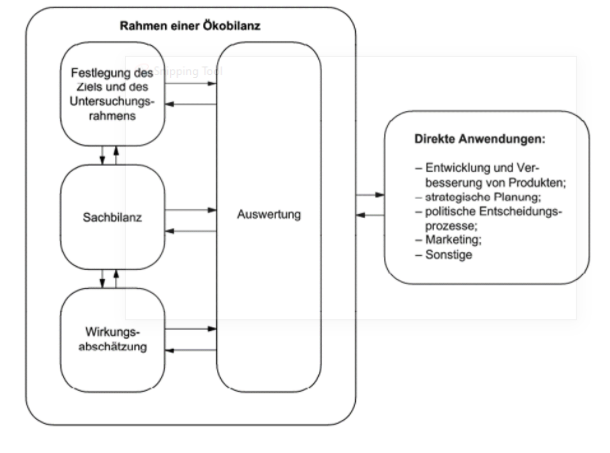
\includegraphics[width=.75\textwidth]{quellen/oekobilanz.png}
    \caption[Phasen einer Ökobilanz]{Phasen einer Ökobilanz (\textit{DIN EN ISO 14040:2009-11}, S.16)}
\end{figure}
\FloatBarrier